% vim: set spell spelllang=en tw=100 et sw=4 sts=4 foldmethod=marker foldmarker={{{,}}} :

\documentclass{beamer}

\usepackage{tikz}
\usepackage{xcolor}
\usepackage{complexity}
\usepackage{hyperref}
\usepackage{microtype}
\usepackage{amsmath}                   % \operatorname
\usepackage{amsfonts}                  % \mathcal
\usepackage{amssymb}                   % \nexists
\usepackage{gnuplot-lua-tikz}          % graphs
\usepackage[vlined]{algorithm2e} % algorithms
\usepackage{centernot}
\usepackage{mathtools}
\usepackage{listings}

\usetikzlibrary{shapes, arrows, shadows, calc, positioning, fit}
\usetikzlibrary{decorations.pathreplacing, decorations.pathmorphing, shapes.misc}
\usetikzlibrary{tikzmark}

\definecolor{uofguniversityblue}{rgb}{0, 0.219608, 0.396078}

\definecolor{uofgheather}{rgb}{0.356863, 0.32549, 0.490196}
\definecolor{uofgaquamarine}{rgb}{0.603922, 0.72549, 0.678431}
\definecolor{uofgslate}{rgb}{0.309804, 0.34902, 0.380392}
\definecolor{uofgrose}{rgb}{0.823529, 0.470588, 0.709804}
\definecolor{uofgmocha}{rgb}{0.709804, 0.564706, 0.47451}
\definecolor{uofgsandstone}{rgb}{0.321569, 0.278431, 0.231373}
\definecolor{uofgforest}{rgb}{0, 0.2, 0.129412}
\definecolor{uofglawn}{rgb}{0.517647, 0.741176, 0}
\definecolor{uofgcobalt}{rgb}{0, 0.615686, 0.92549}
\definecolor{uofgturquoise}{rgb}{0, 0.709804, 0.819608}
\definecolor{uofgsunshine}{rgb}{1.0, 0.862745, 0.211765}
\definecolor{uofgpumpkin}{rgb}{1.0, 0.72549, 0.282353}
\definecolor{uofgthistle}{rgb}{0.584314, 0.070588, 0.447059}
\definecolor{uofgrust}{rgb}{0.603922, 0.227451, 0.023529}
\definecolor{uofgburgundy}{rgb}{0.490196, 0.133333, 0.223529}
\definecolor{uofgpillarbox}{rgb}{0.701961, 0.047059, 0}
\definecolor{uofglavendar}{rgb}{0.356863, 0.301961, 0.580392}

\tikzset{vertex/.style={draw, circle, inner sep=0pt, minimum size=0.5cm, font=\small\bfseries}}
\tikzset{notvertex/.style={vertex, color=white, text=black}}
\tikzset{plainvertex/.style={vertex}}
\tikzset{vertexc1/.style={vertex, fill=uofgburgundy, text=white}}
\tikzset{vertexc2/.style={vertex, fill=uofgsandstone, text=white}}
\tikzset{vertexc3/.style={vertex, fill=uofgforest, text=white}}
\tikzset{vertexc4/.style={vertex, fill=uofgheather, text=white}}
\tikzset{edge/.style={color=black!50!white}}
\tikzset{bedge/.style={ultra thick}}
\tikzset{edged/.style={color=screengrey, dashed}}
\tikzset{edgel3/.style={color=uofgrose, ultra thick}}

% {{{ theme things
\useoutertheme[footline=authortitle]{miniframes}
\useinnertheme{rectangles}

\setbeamerfont{block title}{size={}}
\setbeamerfont{title}{size=\large,series=\bfseries}
\setbeamerfont{section title}{size=\large,series=\mdseries}
\setbeamerfont{author}{size=\normalsize,series=\mdseries}
\setbeamercolor*{structure}{fg=uofguniversityblue}
\setbeamercolor*{palette primary}{use=structure,fg=black,bg=white}
\setbeamercolor*{palette secondary}{use=structure,fg=white,bg=uofgcobalt}
\setbeamercolor*{palette tertiary}{use=structure,fg=white,bg=uofguniversityblue}
\setbeamercolor*{palette quaternary}{fg=white,bg=black}

\setbeamercolor*{titlelike}{parent=palette primary}

\beamertemplatenavigationsymbolsempty

\setbeamertemplate{title page}
{
    \begin{tikzpicture}[remember picture, overlay]
        \node at (current page.north west) {
            \begin{tikzpicture}[remember picture, overlay]
                \fill [fill=uofguniversityblue, anchor=north west] (0, 0) rectangle (\paperwidth, -2.6cm);
            \end{tikzpicture}
        };

        \node (logo) [anchor=north east, shift={(-0.6cm,-0.6cm)}] at (current page.north east) {
            \includegraphics*[keepaspectratio=true,scale=0.7]{UoG_keyline.pdf}
        };

        \node [anchor=west, xshift=0.2cm] at (current page.west |- logo.west) {
            \begin{minipage}{0.65\paperwidth}\raggedright
                {\usebeamerfont{title}\usebeamercolor[white]{}\inserttitle}\\[0.1cm]
                {\usebeamerfont{author}\usebeamercolor[white]{}\insertauthor}
            \end{minipage}
        };
    \end{tikzpicture}
}

\setbeamertemplate{section page}
{
    \begin{centering}
        \begin{beamercolorbox}[sep=12pt,center]{part title}
            \usebeamerfont{section title}\insertsection\par
        \end{beamercolorbox}
    \end{centering}
}

\newcommand{\frameofframes}{/}
\newcommand{\setframeofframes}[1]{\renewcommand{\frameofframes}{#1}}

\makeatletter
\setbeamertemplate{footline}
{%
    \begin{beamercolorbox}[colsep=1.5pt]{upper separation line foot}
    \end{beamercolorbox}
    \begin{beamercolorbox}[ht=2.5ex,dp=1.125ex,%
        leftskip=.3cm,rightskip=.3cm plus1fil]{author in head/foot}%
        \leavevmode{\usebeamerfont{author in head/foot}\insertshortauthor}%
        \hfill%
        {\usebeamerfont{institute in head/foot}\usebeamercolor[fg]{institute in head/foot}\insertshortinstitute}%
    \end{beamercolorbox}%
    \begin{beamercolorbox}[ht=2.5ex,dp=1.125ex,%
        leftskip=.3cm,rightskip=.3cm plus1fil]{title in head/foot}%
        {\usebeamerfont{title in head/foot}\insertshorttitle}%
        \hfill%
        {\usebeamerfont{frame number}\usebeamercolor[fg]{frame number}\insertframenumber~\frameofframes~\inserttotalframenumber}
    \end{beamercolorbox}%
    \begin{beamercolorbox}[colsep=1.5pt]{lower separation line foot}
    \end{beamercolorbox}
}

% }}}

\title{Parallel Search}
\author[Ciaran McCreesh and Patrick Prosser]{\textbf{Ciaran McCreesh} and Patrick Prosser}

\begin{document}

{
    \usebackgroundtemplate{
        \tikz[overlay, remember picture]
        \node[at=(current page.south), anchor=south, inner sep=0pt]{\includegraphics*[keepaspectratio=true, width=\paperwidth]{background4.jpg}};
    }
    \begin{frame}[plain,noframenumbering]
        \titlepage
    \end{frame}
}

\begin{frame}{This Week's Lectures}
    \begin{itemize}
        \item Search and Discrepancies
        \item Parallel Constraint Programming
        \item \textcolor{uofgcobalt}{Parallel Search}
            \begin{itemize}
                \item Embarrassingly Parallel Search
                \item Work stealing
                \item Confidence Based Work Stealing
            \end{itemize}
    \end{itemize}
\end{frame}

\begin{frame}{Fixed Parallel Tree Search, Again}

    \begin{center}
        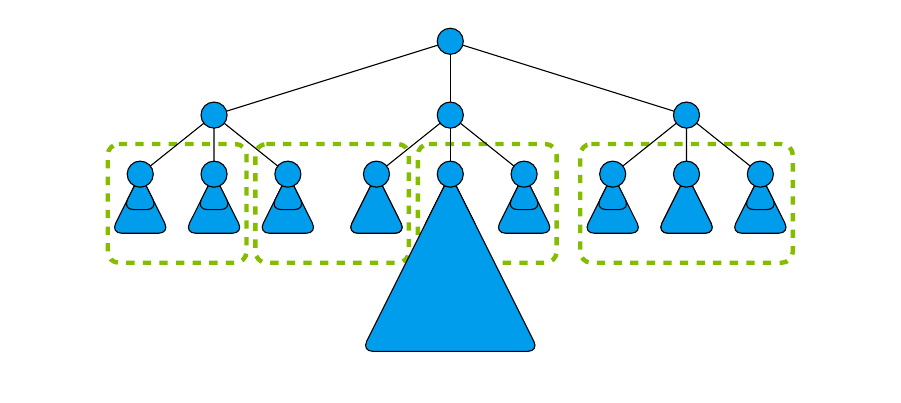
\begin{tikzpicture}[scale=0.75]%{{{
        \coordinate (R);

        \coordinate (N) at (R);

        \coordinate (N1) at ($(N) + (-4, -1.25)$);
        \coordinate (N2) at ($(N) + ( 0, -1.25)$);
        \coordinate (N3) at ($(N) + ( 4, -1.25)$);

        \foreach \na in {1, ..., 3}{
            \coordinate (N\na 1) at ($(N\na) + (-1.25, -1)$);
            \coordinate (N\na 2) at ($(N\na) + ( 0,    -1)$);
            \coordinate (N\na 3) at ($(N\na) + ( 1.25, -1)$);

            \foreach \nb in {1, ..., 3}{
                \coordinate (N\na\nb t1) at ($(N\na\nb) + (-0.5, -1)$);
                \coordinate (N\na\nb t2) at ($(N\na\nb) + ( 0.5, -1)$);

                \coordinate (N\na\nb s1) at ($(N\na\nb) + (-0.3, -0.6)$);
                \coordinate (N\na\nb s2) at ($(N\na\nb) + ( 0.3, -0.6)$);

                \coordinate (N\na\nb h1) at ($(N\na\nb) + (-1.5, -3)$);
                \coordinate (N\na\nb h2) at ($(N\na\nb) + ( 1.5, -3)$);
            }
        }

        \tikzstyle{p} = [draw, rounded corners, dashed, color=uofglawn, ultra thick];
        \draw <2-3> [p] ($(N11) + (-0.55, 0.51)$) -- ($(N12) + (0.55, 0.51)$) -- ($(N12) + (0.55, -1.5)$) -- ($(N11) + (-0.55, -1.5)$) -- cycle;
        \draw <2-3> [p] ($(N13) + (-0.55, 0.51)$) -- ($(N21) + (0.55, 0.51)$) -- ($(N21) + (0.55, -1.5)$) -- ($(N13) + (-0.55, -1.5)$) -- cycle;
        \draw <2-3> [p] ($(N22) + (-0.55, 0.51)$) -- ($(N23) + (0.55, 0.51)$) -- ($(N23) + (0.55, -1.5)$) -- ($(N22) + (-0.55, -1.5)$) -- cycle;
        \draw <2-3> [p] ($(N31) + (-0.55, 0.51)$) -- ($(N33) + (0.55, 0.51)$) -- ($(N33) + (0.55, -1.5)$) -- ($(N31) + (-0.55, -1.5)$) -- cycle;

        \foreach \na in {1, ..., 3}{
            \draw (N) -- (N\na);
            \foreach \nb in {1, ..., 3}{
                \draw (N\na) -- (N\na\nb);
            }
        }

        \tikzstyle{t} = [draw, fill, fill=uofgcobalt, rounded corners];
        \foreach \na in {1, ..., 3}{
            \foreach \nb in {1, ..., 3}{
                \draw <1-2> [t] (N\na\nb) -- (N\na\nb t1) -- (N\na\nb t2) -- cycle;
            }
        }

        \draw <3> [t] (N11) -- (N11s1) -- (N11s2) -- cycle;
        \draw <3> [t] (N12) -- (N12s1) -- (N12s2) -- cycle;
        \draw <3> [t] (N13) -- (N13s1) -- (N13s2) -- cycle;

        \draw <3> [t] (N21) -- (N21t1) -- (N21t2) -- cycle;
        \draw <3> [t] (N22) -- (N22h1) -- (N22h2) -- cycle;
        \draw <3> [t] (N23) -- (N23s1) -- (N23s2) -- cycle;

        \draw <3> [t] (N31) -- (N31s1) -- (N31s2) -- cycle;
        \draw <3> [t] (N32) -- (N32t1) -- (N32t2) -- cycle;
        \draw <3> [t] (N33) -- (N33s1) -- (N33s2) -- cycle;

        \tikzstyle{c} = [draw, circle, fill, fill=uofgcobalt];
        \node [c] at (N) { };

        \foreach \na in {1, ..., 3}{
            \node [c] at (N\na) { };

            \foreach \nb in {1, ..., 3}{
                \node [c] at (N\na\nb) { };
            }
        }

        \node at (-7, -5.5) { }; \node at (7, -5.5) { };
    \end{tikzpicture}%}}}
    \end{center}
\end{frame}

\begin{frame}{What We Need}
    \begin{itemize}
        \item We need a large parallelisable portion of the algorithm, \emph{and} good work
            balance, or we don't get much of an improvement.
    \end{itemize}
\end{frame}

\begin{frame}{Embarrassingly Parallel Search}
    \only<1>{
        \begin{itemize}
            \item If we create $n$ subproblems, chances are we'll get poor balance.
            \item We can't tell beforehand where the really hard subproblems will be.
            \item What if we create \emph{lots} of subproblems?
        \end{itemize}
    }
\end{frame}

\begin{frame}{Work Stealing}
    \begin{itemize}
        \item What if we split work entirely dynamically?
        \item Whenever a worker is idle, have it steal a subproblem from another worker.
    \end{itemize}
\end{frame}

\begin{frame}{Speedups from Parallel Tree Search}

    \only<1>{
        \begin{itemize}
            \item If a decision problem is satisfiable, or for an optimisation problem, our speedups
                could be arbitrary: one worker might find a feasible or strong solution very quickly. In
                particular, \emph{superlinear} speedups are possible, as are no speedups at all.

            \item For an unsatisfiable decision problem, or for an enumeration problem, our speedups
                can be at best linear (assuming we do not change the search tree): we \emph{are}
                dividing up a fixed amount of work.

            \item If we do not communicate bounds, or if we do not preserve sequential ordering, we
                could get an \emph{absolute slowdown}.
        \end{itemize}
    }
\end{frame}

\begin{frame}{Work Splitting Affects Search}

    \only<1-3>{
        \begin{center}
            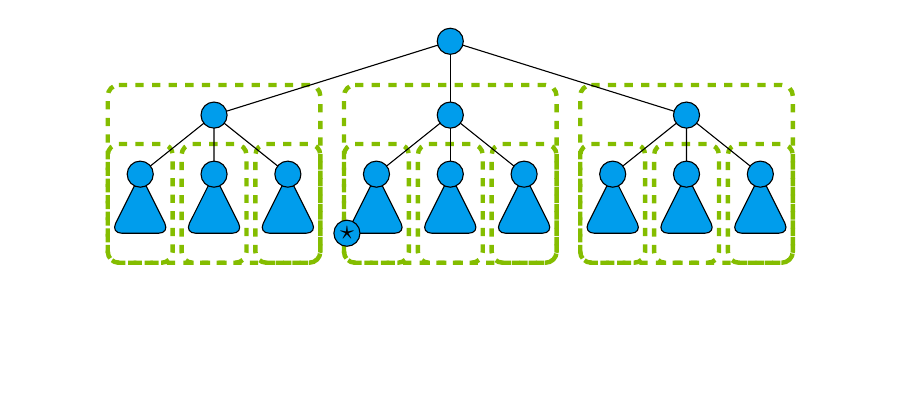
\begin{tikzpicture}[scale=0.75]%{{{
            \coordinate (R);

            \coordinate (N) at (R);

            \coordinate (N1) at ($(N) + (-4, -1.25)$);
            \coordinate (N2) at ($(N) + ( 0, -1.25)$);
            \coordinate (N3) at ($(N) + ( 4, -1.25)$);

            \foreach \na in {1, ..., 3}{
                \coordinate (N\na 1) at ($(N\na) + (-1.25, -1)$);
                \coordinate (N\na 2) at ($(N\na) + ( 0,    -1)$);
                \coordinate (N\na 3) at ($(N\na) + ( 1.25, -1)$);

                \foreach \nb in {1, ..., 3}{
                    \coordinate (N\na\nb t1) at ($(N\na\nb) + (-0.5, -1)$);
                    \coordinate (N\na\nb t2) at ($(N\na\nb) + ( 0.5, -1)$);

                    \coordinate (N\na\nb s1) at ($(N\na\nb) + (-0.3, -0.6)$);
                    \coordinate (N\na\nb s2) at ($(N\na\nb) + ( 0.3, -0.6)$);

                    \coordinate (N\na\nb h1) at ($(N\na\nb) + (-1.5, -3)$);
                    \coordinate (N\na\nb h2) at ($(N\na\nb) + ( 1.5, -3)$);
                }
            }

            \tikzstyle{p} = [draw, rounded corners, dashed, color=uofglawn, ultra thick];
            \foreach \na in {1, ..., 3}{
                \foreach \nb in {1, ..., 3}{
                    \draw <1-2> [p] ($(N\na\nb) + (-0.55, 0.51)$) -- ($(N\na\nb) + (0.55, 0.51)$) --
                        ($(N\na\nb) + (0.55, -1.5)$) -- ($(N\na\nb) + (-0.55, -1.5)$) -- cycle;
                }

                \draw <3> [p] ($(N\na 1) + (-0.55, 1.51)$) -- ($(N\na 3) + (0.55, 1.51)$) --
                    ($(N\na 3) + (0.55, -1.5)$) -- ($(N\na 1) + (-0.55, -1.5)$) -- cycle;
            }

            \foreach \na in {1, ..., 3}{
                \draw (N) -- (N\na);
                \foreach \nb in {1, ..., 3}{
                    \draw (N\na) -- (N\na\nb);
                }
            }

            \tikzstyle{t} = [draw, fill, fill=uofgcobalt, rounded corners];
            \foreach \na in {1, ..., 3}{
                \foreach \nb in {1, ..., 3}{
                    \draw [t] (N\na\nb) -- (N\na\nb t1) -- (N\na\nb t2) -- cycle;
                }
            }

            \tikzstyle{c} = [draw, circle, fill, fill=uofgcobalt];
            \node [c] at (N) { };

            \foreach \na in {1, ..., 3}{
                \node [c] at (N\na) { };

                \foreach \nb in {1, ..., 3}{
                    \node [c] at (N\na\nb) { };
                }
            }

            \node <2-3> [c] at (N21t1) { };
            \node <2-3> at (N21t1) { $\star$ };

            \node at (-7, -5.5) { }; \node at (7, -5.5) { };
        \end{tikzpicture}%}}}
        \end{center}
    }

    \only<4>{
        \begin{itemize}
            \item For satisfiable instances and optimisation problems, where you split the work doesn't just
                affect balance. It also affects the amount of work to do. We just saw an example where
                \emph{better} work balance gave \emph{worse} performance, because it took longer to
                find a solution.

            \item Remember Harvey and Ginsberg, from Monday?

                \begin{enumerate}\stepcounter{enumi}
                    \item Value-ordering heuristics are most likely to wrong higher up in the tree (there is
                        least information available when no or few choices have been made).
                \end{enumerate}

            \item Stealing early or splitting high introduces diversity against early heuristic
                choices. Stealing late gives a close-to-sequential ordering.
        \end{itemize}
    }

\end{frame}

\begin{frame}{Confidence Based Work Stealing}

\end{frame}

\begin{frame}{This is Not The Exam Question}
    Suppose we are solving a decision problem which has a sequential part taking
    one second to run, and a parallelisable part which takes twenty seconds to run on one
    processor. What is the best possible runtime we might see when using ten processors to
    solve this problem with a parallel tree-search, if the instance is satisfiable? What if
    it is unsatisfiable?
\end{frame}

\begin{frame}[plain,noframenumbering]
    \begin{tikzpicture}[remember picture, overlay]
        \node at (current page.north west) {
            \begin{tikzpicture}[remember picture, overlay]
                \fill [fill=uofguniversityblue, anchor=north west] (0, 0) rectangle (\paperwidth, -1.7cm);
            \end{tikzpicture}
        };

        \node (logo) [anchor=north east, shift={(-0.3cm,-0.2cm)}] at (current page.north east) {
            \includegraphics*[keepaspectratio=true,scale=0.55]{UoG_keyline.pdf}
        };
    \end{tikzpicture}
\end{frame}

\end{document}

